\documentclass[aspectratio=169,10pt]{beamer}
\usetheme{default}
\usecolortheme{seagull}
\setbeamertemplate{navigation symbols}{}
\setbeamertemplate{footline}[frame number]
\setbeamerfont{frametitle}{series=\bfseries,size=\large}
\setbeamercolor{frametitle}{fg=black}
\usepackage{tikz,booktabs,amsmath,amssymb}
\usetikzlibrary{positioning,arrows.meta,fit,calc,backgrounds}

% validated categorical palette (light mode)
\definecolor{cblue}{HTML}{2A78D6}
\definecolor{caqua}{HTML}{1BAF7A}
\definecolor{cyellow}{HTML}{EDA100}
\definecolor{cgreen}{HTML}{008300}
\definecolor{cviolet}{HTML}{4A3AA7}
\definecolor{cred}{HTML}{E34948}
\definecolor{cgray}{HTML}{52514E}
\definecolor{cpale}{HTML}{E8E7E2}

\newcommand{\claim}[1]{\textcolor{cviolet}{\textbf{Claim:} #1}}
\newcommand{\sg}{\mathrm{sg}}

\title{Discourse-JEPA:\\ Latent World Models over Reasoning Steps}
\subtitle{Historical experiment chronology (archival)\\
Paper-facing replacement: \texttt{discourse\_jepa\_neurips.pdf}}
\author{TextJEPA project}
\date{July 13, 2026 \quad (repo: \texttt{TextJEPA/}, runs: \texttt{runs/})}

\begin{document}
\frame{\titlepage}

% ---------------------------------------------------------------- idea
\begin{frame}{Idea in one slide}
\begin{itemize}
  \item Treat a \textbf{reasoning trace} as trajectories of a world model: the
        \emph{state} $s_t$ is a compressed discourse state (``what has been
        established''), the \emph{action} $a_t$ is a tiny latent code of an
        \emph{intent phrase} for the next step.
  \item Actions state intent only (\emph{``derive purple apples from orange
        jars times green pens .''}) --- never the outcome (\emph{``$=5$''}).
        The predictor $F(s_t,a_t)$ must therefore \textbf{compute consequences
        in latent space}.
  \item Generation = \textbf{search over actions}: roll candidate actions
        forward with $F$, score with an energy, execute the best in the
        environment, re-encode, replan (closed-loop MPC). The world model
        predicts \textbf{latents, not outcome tokens}; an optional training-only
        LDAD head reconstructs the observed action phrase and is discarded at
        planning time.
  \item Synthetic reasoning world $\Rightarrow$ exact ground truth for
        \textbf{linear probes} and \textbf{objective planning success}.
\end{itemize}
\end{frame}

\begin{frame}{Research questions and current answers}
\begin{enumerate}\itemsep4pt
  \item \textbf{A latent world model over reasoning steps works} --- and we
        can \emph{audit} it: predicted futures of never-taken actions match
        symbolic execution (Results 1, 2, 9).
  \item \textbf{What silently breaks}: jointly learned encoders can discard
        computed content to simplify prediction (Result 3); latent distance is not
        a progress metric (Result 5).
  \item \textbf{Reconstruction-free fixes}: frozen random-init embedding
        targets restore content (Result 4); trajectory-geometry losses fix
        the metric (Results 7, 8); counterfactual \emph{ranking} fixes the
        energy's discrimination (Result 10).
  \item \textbf{The energy can come from the geometry itself}: a value head
        distilled from latent goal distance, without scalar distance-to-go
        labels, matches the scalar-supervised alternative within seed variance
        (Results 13, 16).
  \item \textbf{Baselines and limits}: likelihood selection (LMs at any
        tested scale/granularity) clusters far below (Result 15); failures
        are chain-depth-limited --- the scale-up frontier (Result 16).
\end{enumerate}
\end{frame}

\begin{frame}{Notation and experimental terminology}
\footnotesize
\begin{tabular}{p{0.29\textwidth}p{0.67\textwidth}}
\toprule
\textbf{discourse state} $s_t$ & one vector summarizing prompt + steps
  $1..t$ (output of the causal state model)\\
\textbf{predictor} $F(s,a)$ & MLP producing the next state from state +
  action code (the world model)\\
\textbf{action} $a$ & 16-d encoding of an \emph{intent phrase} ("derive X
  from Y times Z") --- states what to do, never the outcome\\
\textbf{value head} $V(s, s_0)$ & scalar energy: estimated necessary steps
  remaining; the planner minimizes steps${}+V$\\
\textbf{end-to-end value shaping} & value-head gradients enter the encoder
  so the planning energy can shape the representation\\
\textbf{observed-action displacement decoding} & reconstruct the complete
  observed intent-token sequence from $\Delta s=s_{t+1}-s_t$; our historical
  hybrid operation/embedding target is reported only as a distinct control\\
\textbf{fixed outcome target} & predict a frozen random-feature embedding
  of the next sentence; prevents loss-minimizing content deletion\\
\textbf{counterfactual preference loss} & margin loss ordering $V(F(s,a_i))$ over $K$
  counterfactual actions per state by their symbolic outcomes\\
\textbf{cross-horizon cost calibration} & order multi-step costs (depth${}+V$) ---
  calibrates search depth\\
\textbf{goal-monotonicity constraint} & necessary steps must decrease the latent
  distance to the trace-terminal state by a margin\\
\textbf{geometry-distilled value} & value head regressed on that latent goal
  distance (geometry target, no numeric labels)\\
\bottomrule
\end{tabular}

\end{frame}

\begin{frame}{Scientific labels and artifact identifiers}
\small
Artifact names are retained only for reproducibility; the report uses the
scientific labels in the left column.
\medskip
\centering
\begin{tabular}{p{0.47\textwidth}p{0.42\textwidth}}
\toprule
scientific label & repository artifact\\
\midrule
fixed-outcome prediction + end-to-end value shaping & \texttt{disc\_combo}\\
goal-monotone value regression & \texttt{disc\_mono\_hi}\\
counterfactual preference learning ($K=2$) & \texttt{disc\_rank\_k2}\\
geometry-distilled counterfactual model & \texttt{disc\_mono\_distill\_rank}\\
five-objective ranked JEPA & \texttt{disc\_core5}\\
cross-horizon calibrated model & suffix \texttt{\_cal}\\
independent seed replicates & suffixes \texttt{\_s2}, \texttt{\_s3}\\
\bottomrule
\end{tabular}

\medskip
The five-objective model uses one-step latent prediction, counterfactual
preference learning, VICReg, fixed outcome targets, and displacement decoding.
The ``full'' model additionally uses rollout, hierarchy, and goal-geometry terms.
\end{frame}

\begin{frame}{Headline comparison: fixed one-step planning protocol}
\claim{Under identical one-step MPC, the five-objective ranked JEPA improves
strict-budget success by 14.5 points over the largest token LM tested.}
\centering\small
\begin{tabular}{lcc}
\toprule
 & @optimal & @slack-2\\
\midrule
random feasible policy & 0.055 & 0.405\\
token LM, parameter-matched (best lr) & 0.670 & 0.910\\
token LM, $3\times$ larger & 0.735 & 0.940\\
\textbf{five-objective ranked JEPA} & \textbf{0.880 $\pm$ 0.004}
 & \textbf{0.975 $\pm$ 0.004}\\
geometry-distilled ranked JEPA & 0.900 $\pm$ 0.027 & 0.980 $\pm$ 0.008\\
symbolic oracle & 1.00 & 1.00\\
\bottomrule
\end{tabular}

\medskip
All learned rows use greedy lookahead 1 and the same 200 validation episodes.
The five-objective model's value head is trained by pairwise margins, without
scalar remaining-step labels. Mean $\pm$ standard deviation uses three seeds.
\end{frame}

\begin{frame}{Search-depth interaction is a separate experiment}
\claim{Cross-horizon calibration helps the full model, but not the
five-objective model; it is not a generic ``depth option.''}
\centering\small
\begin{tabular}{lccc}
\toprule
training objective & lookahead 1 & lookahead 2 & slack-2, lookahead 2\\
\midrule
five-objective + cross-horizon calibration & 0.900 & 0.885 & 0.985\\
full geometry-distilled + cross-horizon calibration & 0.925 & \textbf{0.945} & \textbf{1.000}\\
\bottomrule
\end{tabular}

\medskip\footnotesize
The five-objective model combines latent prediction, fixed outcome prediction,
VICReg, displacement decoding, and pairwise preferences. The full
geometry-distilled model additionally shapes goal-distance monotonicity and
distills that distance into $V$. Single-seed interaction test.
``Cross-horizon'' means that training compares
$1+V(F(s,a))$ with $2+V(F(F(s,a),a'))$; ``lookahead'' is the matching
planning-time rollout depth. This is not part of the three-seed headline table.
\end{frame}

\begin{frame}{Value-head supervision targets compared (symbolic vs geometric)}
\claim{With matched pairwise preference supervision, geometry-distilled values
match scalar-supervised values within seed variance, provided the geometry is
goal-monotone.}
\centering\small
\begin{tabular}{llccc}
\toprule
$V$ trained on & metric shaping & labels used & @opt & @slack2\\
\midrule
numeric remaining-steps & --- & scalar counts & 0.64$\pm$.05 & 0.89\\
numeric + ranking & --- & counts + order & 0.91$\pm$.03 & 0.99\\
numeric + ranking + hinge & hinge & counts + order + binary & 0.89$\pm$.02 & 0.99\\
\midrule
latent goal distance & \textbf{none} (control) & none & 0.19 & 0.64\\
latent goal distance & curvature (label-free) & none & 0.30 & 0.72\\
latent goal distance & hinge & binary relevance & 0.57$\pm$.05 & 0.89\\
\textbf{lat.\ dist.\ + ranking} & hinge & binary + order & \textbf{0.90$\pm$.03} & \textbf{0.98}\\
\bottomrule
\end{tabular}

\smallskip
Reading: the distilled (geometric) value head is a drop-in replacement for
numeric supervision once the metric it distills is goal-monotone; scalar
count labels contribute nothing beyond binary relevance + ordering
(0.90 vs 0.89/0.91, within seed noise).
\end{frame}

% ---------------------------------------------------------------- data
\begin{frame}{World: iGSM-style synthetic reasoning (exact generator)}
\textbf{Problem sampler} (rejection-sampled until $3\le|\mathcal A_q|\le 9$; \texttt{rng = Random(f"\{seed\}:\{index\}")}):
\begin{itemize}\itemsep1pt
  \item $n\sim\mathcal U\{6,\dots,12\}$ variables; names = distinct
        (adjective, noun) pairs from $20\times 20$ vocabulary.
  \item Variable $i$: with $p{=}0.35$ (always for $i<2$) a \textbf{leaf}
        $x_i = c_i,\ c_i\sim\mathcal U\{0..22\}$; else an \textbf{internal}
        $x_i = x_a \circ x_b \bmod 23$, $\circ\in\{+,-,\times\}$,
        parents $a,b$ sampled from $\{0..i-1\}$.
  \item Query $q$ = uniform over internal variables;
        $\mathcal A_q$ = ancestors of $q$ (incl.\ $q$) = the necessary
        computation; the rest are \textbf{distractors}.
\end{itemize}
\medskip
\textbf{Training traces}: solve by repeatedly resolving a feasible variable
(parents resolved); with $p{=}0.15$ (max 2) pick a feasible \emph{distractor}
instead of a necessary one $\Rightarrow$ off-path states for the value head.
\textbf{Important protocol correction.} Published artifacts in this deck reused
the same deterministic index set each epoch. New runs (July 13 onward) use
disjoint epoch-offset indices, preserving determinism while generating fresh
problems; validation remains fixed.
\end{frame}

\begin{frame}[fragile]{A verbatim sample (val problem \#3)}
\footnotesize
\textbf{Prompt} (definitions shuffled per-sample, question last; one sentence = one chunk):
\begin{quote}\ttfamily
the number of purple apples equals the number of orange jars times the number of green pens .\\
the number of orange jars is 15 . \quad the number of green pens is 8 .\\
\textcolor{cgray}{(+ 7 distractor definitions)} \quad how many purple apples are there ?
\end{quote}
\textbf{Solution trace} --- step sentence (observed outcome) vs.\ action intent phrase (no outcome):
\begin{center}\ttfamily\begin{tabular}{l|l}
step sentence (encoder sees) & intent phrase (action encoder sees)\\\hline
so the number of green pens is 8 . & look up the number of green pens .\\
so the number of orange jars is 15 . & look up the number of orange jars .\\
so the number of purple apples is & derive purple apples from orange\\
\quad 15 times 8 = 5 . & \quad jars times green pens .
\end{tabular}\end{center}
\smallskip
Note $15\times 8 = 120 \equiv 5 \pmod{23}$: outcomes are nontrivial to predict.
\end{frame}

% ---------------------------------------------------------------- architecture
\begin{frame}{Architecture (all sizes exact; 8.8--9.1M params)}
\begin{itemize}\itemsep2pt
  \item \textbf{Chunk encoder} $E_c$: word-level vocab (441 tokens), embed 256,
        2-layer pre-norm transformer (4 heads, FF 1024), masked mean-pool
        $\to$ one 256-d vector per sentence. Shared for prompt, steps, intents.
  \item \textbf{State model} $E_s$: 4-layer \emph{causal} transformer
        (8 heads, FF 1024) over [prompt chunks $|$ step chunks] + learned
        positions + 2 segment embeddings. $s_0$ = hidden at the question;
        $s_t$ = hidden at step $t$.
  \item \textbf{Action encoder} $A$: MLP $256\to256\to16$ on the intent-phrase
        embedding (optional FSQ, unused in main runs).
  \item \textbf{Predictor} $F$: residual MLP,
        $\hat s_{t+1}=s_t+\mathrm{MLP}([\mathrm{LN}(s_t);a_t])$, 2 hidden
        layers of 1024 (GELU).
  \item \textbf{Hierarchy}: CLS-transformer over $K{=}3$ action codes
        $\to$ 8-d macro action $m_t$; $F_{\mathrm{hi}}(s_t,m_t)$ predicts
        $\bar s_{t+3}$ (same latent space, HWM-style).
  \item \textbf{Observed-action displacement decoder}: position-query
        transformer on $\Delta s=s_{t+1}-s_t$ reconstructs the complete intent
        phrase. The historical hybrid head (operation class + EMA intent
        embedding) is not a faithful Delta-JEPA target.
  \item \textbf{Value head} $V$: MLP on $[\mathrm{LN}([s_t;s_0])]$
        $\to$ scalar = predicted remaining necessary steps.
  \item \textbf{Teachers}: EMA copies of $E_c,E_s$ (momentum $0.99\to0.999$
        linear); \textbf{frozen anchor} $\tilde E_c$ = copy of $E_c$ at random
        init, never updated.
\end{itemize}
\end{frame}

\begin{frame}{Training pipeline}
\centering
\resizebox{0.94\textwidth}{!}{%
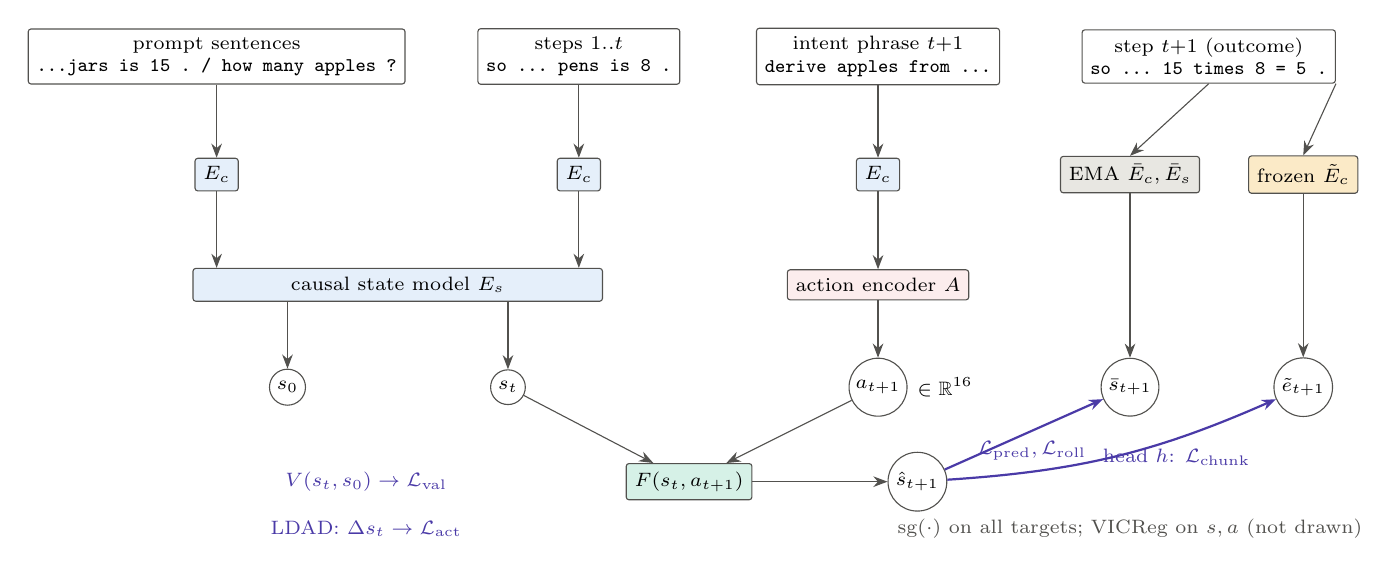
\begin{tikzpicture}[font=\scriptsize,
  box/.style={draw=cgray, rounded corners=1pt, inner sep=3pt, align=center},
  enc/.style={box, fill=cblue!12},
  tgt/.style={box, fill=cpale},
  frz/.style={box, fill=cyellow!22},
  act/.style={box, fill=cred!10},
  lat/.style={circle, draw=cgray, inner sep=1.6pt, fill=white},
  loss/.style={align=center, text=cviolet, font=\scriptsize},
  arr/.style={-{Stealth[length=1.8mm]}, cgray}]

% ---- column x positions: 0, 42, 84, 126 (mm-ish units)
% sentences row (y=0)
\node[box] (p)  at (0,0)   {prompt sentences\\ \ttfamily ...jars is 15 .\ / how many apples ?};
\node[box] (y1) at (4.6,0) {steps $1..t$\\ \ttfamily so ...\ pens is 8 .};
\node[box] (u)  at (8.4,0) {intent phrase $t{+}1$\\ \ttfamily derive apples from ...};
\node[box] (y2) at (12.6,0){step $t{+}1$ (outcome)\\ \ttfamily so ...\ 15 times 8 = 5 .};

% encoder row (y=-1.4)
\node[enc] (ecp) at (0,-1.5)   {$E_c$};
\node[enc] (ecy) at (4.6,-1.5) {$E_c$};
\node[enc] (ecu) at (8.4,-1.5) {$E_c$};
\node[tgt] (ema) at (11.6,-1.5){EMA $\bar E_c,\bar E_s$};
\node[frz] (frz) at (13.8,-1.5){frozen $\tilde E_c$};

% state model row
\node[enc, minimum width=52mm] (es) at (2.3,-2.9) {causal state model $E_s$};
\node[act] (ae) at (8.4,-2.9) {action encoder $A$};

% latent row
\node[lat] (s0) at (0.9,-4.2) {$s_0$};
\node[lat] (st) at (3.7,-4.2) {$s_t$};
\node[lat, label={[font=\scriptsize]right:{$\in\mathbb R^{16}$}}] (a) at (8.4,-4.2) {$a_{t+1}$};
\node[lat] (sbar) at (11.6,-4.2) {$\bar s_{t+1}$};
\node[lat] (ce)   at (13.8,-4.2) {$\tilde e_{t+1}$};

% predictor row
\node[box, fill=caqua!18] (F) at (6.0,-5.4) {$F(s_t,a_{t+1})$};
\node[lat] (shat) at (8.9,-5.4) {$\hat s_{t+1}$};

\draw[arr] (p) -- (ecp); \draw[arr] (y1) -- (ecy); \draw[arr] (u) -- (ecu);
\draw[arr] (y2.south) -- (ema.north); \draw[arr] (y2.south east) -- (frz.north);
\draw[arr] (ecp) -- (ecp |- es.north); \draw[arr] (ecy) -- (ecy |- es.north);
\draw[arr] (ecu) -- (ae);
\draw[arr] (s0 |- es.south) -- (s0); \draw[arr] (st |- es.south) -- (st);
\draw[arr] (ae) -- (a);
\draw[arr] (ema) -- (sbar); \draw[arr] (frz) -- (ce);
\draw[arr] (st) -- (F); \draw[arr] (a) -- (F);
\draw[arr] (F) -- (shat);

\draw[arr, cviolet, thick] (shat) -- node[below, loss, pos=0.55]
  {$\mathcal L_{\text{pred}},\mathcal L_{\text{roll}}$} (sbar);
\draw[arr, cviolet, thick] (shat) to[bend right=10]
  node[below, loss, pos=0.7]{head $h$: $\mathcal L_{\text{chunk}}$} (ce);

\node[loss] at (1.9,-5.4) {$V(s_t,s_0)\to\mathcal L_{\text{val}}$};
\node[loss] at (1.9,-6.0) {LDAD: $\Delta s_t \to \mathcal L_{\text{act}}$};
\node[loss, text=cgray] at (11.6,-6.0)
  {sg$(\cdot)$ on all targets; VICReg on $s,a$ (not drawn)};
\end{tikzpicture}}
\end{frame}

\begin{frame}{Objectives (exact losses and weights)}
Let $d(x,y)=\mathrm{smoothL1}(\mathrm{LN}(x),\mathrm{LN}(y))$ (per-dim mean;
LN = parameter-free layer norm), masks over valid steps.
\begin{align*}
\mathcal L_{\text{pred}} &= d\big(F(s_t,a_t),\, \sg\,\bar s_{t+1}\big)
  &\text{weight } 1.0\\
\mathcal L_{\text{roll}} &= d\big(F^{(t)}(s_0,a_{1:t}),\, \sg\,\bar s_{t}\big)
  \ \text{(open loop, all $t$)} &1.0\\
\mathcal L_{\text{hi}} &= d\big(F_{\mathrm{hi}}(s_t, m_t),\, \sg\,\bar s_{t+3}\big)
  &0.5\\
\mathcal L_{\text{vic}} &= \textstyle\sum_j \max(0, 1-\mathrm{std}(s^{(j)}))
  + 0.04\,\|\mathrm{offdiag}(\mathrm{Cov}(s))\|_F^2/D + 0.1\,\text{var}(a)
  &1.0\\
\mathcal L_{\text{obs-act}} &= \mathrm{CE}\big(D(\Delta s_t),\,
  \mathrm{tokens}(u_t)\big)\quad\text{(faithful observed-action LDAD)}
  &\text{0 / selected}\\
\mathcal L_{\text{val}} &= \mathrm{smoothL1}\big(V(s_t,s_0),\,
  \#\text{unresolved necessary}\big) &1.0\\
\mathcal L_{\text{chunk}} &= d\big(h(\hat s_{t+1}),\, \sg\,\tilde E_c(y_{t+1})\big)
  + 0.5\, d\big(h(\text{rollout}_t),\, \sg\,\tilde E_c(y_t)\big)
  &\text{0 / 2.0}\\
\mathcal L_{\text{curv}} &= 1-\cos(v_t,\,v_{t+1}),\quad v_t = s_{t+1}-s_t
  \ \text{(straightening, arXiv:2603.12231)} &\text{0 / .02--.1}\\
\mathcal L_{\text{mono}} &= \mathbb 1_{\text{nec}}\,[\Delta d^{\text{goal}}_t
  + m]_+ + \tfrac12(1-\mathbb 1_{\text{nec}})\,[-\Delta d^{\text{goal}}_t]_+
  &\text{0 / 1--2}
\end{align*}
$\mathcal L_{\text{chunk}}$: weight 0 in \texttt{base}; 2.0 in
\texttt{chunkpred}/\texttt{combo} (\textbf{frozen} anchor
$\tilde E_c$). Value head input detached except
\texttt{valgrad}/\texttt{combo}. $d^{\text{goal}}_t$ = LN-L1 distance
of $s_t$ to the trace-terminal EMA state; margin $m\in\{.02,.05\}$.
\end{frame}

\begin{frame}{Training protocol}
\begin{itemize}\itemsep2pt
  \item AdamW, lr $3\!\times\!10^{-4}$, weight decay $0.05$ (none for dim
        $<2$ params), $\beta=(0.9,0.95)$; cosine schedule to floor $0.05$,
        1000-step warmup; grad clip 5.0.
  \item Batch 128 problems; 20 epochs $\times$ 781 steps at the 100k setting.
        Historical results reused a deterministic 100k corpus. Future runs use
        a deterministic disjoint corpus per epoch. EMA momentum
        $0.99\to0.999$ linear over training.
  \item Hardware: one V100-32GB, fp32, $\sim$40 min/run.
  \item In-training eval each epoch: all losses + collapse diagnostics
        (per-dim std, RankMe effective rank) + closed-form ridge probes.
  \item Code: \texttt{scripts/train.py +experiment=...}; every run's exact
        config is stored in its checkpoint.
\end{itemize}
\end{frame}

% ---------------------------------------------------------------- planning
\begin{frame}{Planning: closed-loop MPC by exhaustive latent search}
\textbf{Interface knowledge} (legitimate): feasible actions = unresolved
variables whose stated dependencies are resolved --- readable from the prompt.
\textbf{Consequence knowledge}: latent only.
\medskip
\begin{enumerate}\itemsep1pt
  \item Encode prompt + steps so far $\to$ $s$ (and $s_0$ once).
  \item Enumerate feasible action \emph{sequences} to depth $L$
        (lookahead; cap 64), encode their intent phrases $\to a_i$.
  \item Roll out $\hat s \leftarrow F(\hat s, a_i)$ along each sequence.
  \item Score: $\;\text{cost} = \text{steps taken} + V(\hat s_{\text{end}},
        s_0)$ \; (estimated total steps).
  \item Execute the first action of the argmin in the symbolic environment
        $\to$ real outcome sentence appended; go to 1.
\end{enumerate}
\medskip
Success = query resolved within the \textbf{strict optimal budget}
$|\mathcal A_q|$ (slack 0: any distractor pick is fatal). 200 val episodes.
Discrete enumeration replaces CEM; a sampled action prior would need CEM/MPPI.
\end{frame}

\begin{frame}{Planning: search graph (one replanning round, lookahead 1)}
\centering
\resizebox{0.8\textwidth}{!}{%
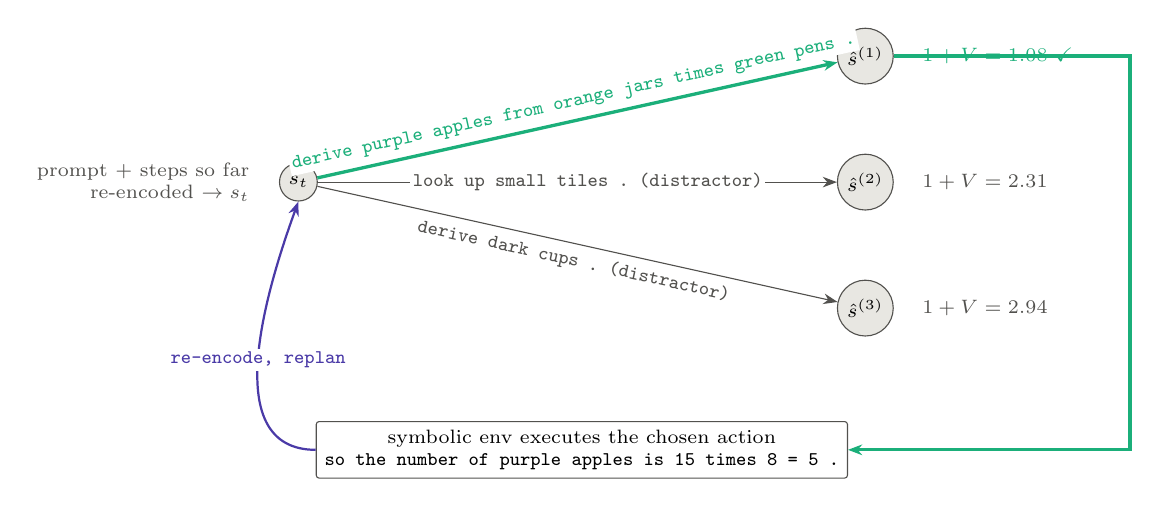
\begin{tikzpicture}[font=\scriptsize,
  lat/.style={circle, draw=cgray, fill=cpale, inner sep=2pt},
  arr/.style={-{Stealth[length=1.8mm]}},
  cand/.style={arr, cgray},
  best/.style={arr, caqua, very thick},
  albl/.style={fill=white, inner sep=1pt, font=\ttfamily\scriptsize}]

\node[lat] (s) at (0,0) {$s_t$};
\node[align=right, text=cgray, anchor=east] at (-0.5,0)
  {prompt + steps so far\\ re-encoded $\to s_t$};

\node[lat] (s1) at (7.2, 1.6) {$\hat s^{(1)}$};
\node[lat] (s2) at (7.2, 0.0) {$\hat s^{(2)}$};
\node[lat] (s3) at (7.2,-1.6) {$\hat s^{(3)}$};

\draw[best] (s) -- node[albl, pos=0.5, above=2pt, sloped]
  {derive purple apples from orange jars times green pens .} (s1);
\draw[cand] (s) -- node[albl, pos=0.52]
  {look up small tiles .\ \textcolor{cgray}{(distractor)}} (s2);
\draw[cand] (s) -- node[albl, pos=0.5, below=2pt, sloped]
  {derive dark cups .\ \textcolor{cgray}{(distractor)}} (s3);

\node[anchor=west, text=caqua] at (7.8, 1.6) {$1+V=1.08$ $\checkmark$};
\node[anchor=west, text=cgray] at (7.8, 0.0) {$1+V=2.31$};
\node[anchor=west, text=cgray] at (7.8,-1.6) {$1+V=2.94$};

\node[draw=cgray, rounded corners=1pt, align=center, inner sep=3pt]
  (env) at (3.6,-3.4)
  {symbolic env executes the chosen action\\
   \ttfamily so the number of purple apples is 15 times 8 = 5 .};
\draw[best] (s1.east) -- ++(3.0,0) |- (env.east);
\draw[arr, cviolet, thick] (env.west) to[out=180,in=-110]
  node[albl, text=cviolet, pos=0.5]{re-encode, replan} (s.south);
\end{tikzpicture}}

\medskip
$V$ values are predicted \emph{remaining necessary steps} of the predicted
next latent; lookahead 2 scores 2-step latent rollouts.
\end{frame}

% ---------------------------------------------------------------- experiments
\begin{frame}{Experiment grid (each condition is one 20-epoch run)}
\centering\small
\resizebox{\textwidth}{!}{%
\begin{tabular}{llll}
\toprule
condition & fixed outcome target & value grad $\to$ encoder & additional change\\
\midrule
latent-prediction reference & --- & no & ---\\
without displacement decoding & --- & no & $\mathcal L_{\text{act}}$ weight 0\\
fixed outcome prediction & frozen, w=2.0 & no & ---\\
end-to-end value shaping & --- & \textbf{yes} & ---\\
fixed outcome + value shaping & frozen, w=2.0 & \textbf{yes} & ---\\
value-only control & --- & \textbf{yes} & \emph{all} JEPA weights 0\\
frozen-encoder control & --- & no & encoders frozen at init\\
\midrule
curvature-weight sweep & frozen, w=2.0 & \textbf{yes}
  & $+\,\mathcal L_{\text{curv}}$, $\lambda\in\{.02,.05,.1\}$\\
goal-monotonicity sweep & frozen, w=2.0 & \textbf{yes}
  & $+\,\mathcal L_{\text{mono}}$, w1\,m.02\,/\,w2\,m.05\\
combined geometric constraints & frozen, w=2.0 & \textbf{yes} & both regularizers\\
monotonicity without value head & frozen, w=2.0 & no
  & $+\,\mathcal L_{\text{mono}}$, \emph{no value head}\\
\midrule
counterfactual preferences ($K=2,4$) & frozen, w=2.0 & \textbf{yes}
  & $+$ ranking over K counterfactual actions\\
preference + goal monotonicity & frozen, w=2.0 & \textbf{yes}
  & ranking K=2 $+$ $\mathcal L_{\text{mono}}$ w2\\
grounding and data controls & frozen, w=2.0 & \textbf{yes}
  & grounding controls (Results 9, 11)\\
\bottomrule
\end{tabular}}

\medskip
Baselines at plan time: \textbf{random feasible policy},
\textbf{symbolic oracle} (=100\%), and \textbf{oracle goal-distance energy}
(LeWM-style, uses the encoded solved state --- diagnostic only).
\end{frame}

\begin{frame}{Result 1 --- historical objective sweep (not an ablation shear)}
\claim{Fixed outcome targets improve the latent baseline; counterfactual
preference learning gives the largest further gain. Adjacent bars are separate
recipes and must not be read as a cumulative one-factor-at-a-time sequence.}
\begin{columns}
\column{0.58\textwidth}
\centering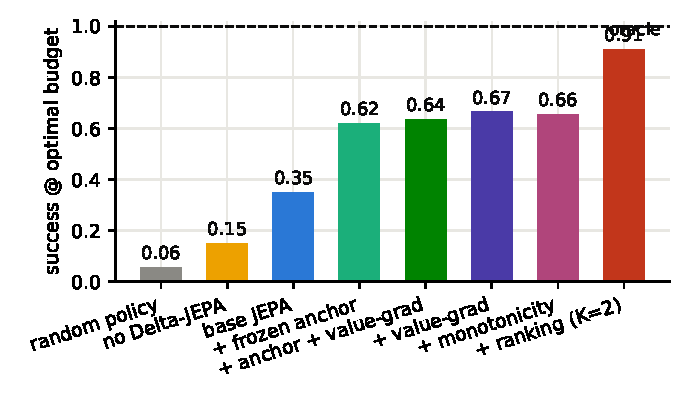
\includegraphics[width=\linewidth]{figs/planning_success.pdf}
\column{0.4\textwidth}\small
Success within the \emph{strict optimal budget}, greedy lookahead 1,
200 episodes, mean necessary steps 4.07.\\[4pt]
With slack 2 (mean of 3 seeds): latent baseline 0.83, fixed outcome target
0.89, goal monotonicity 0.91, counterfactual preference models
\textbf{0.98--0.99} (random 0.41).\\[4pt]
Distractor pick rate: random 0.43 $\to$ latent baseline 0.28 $\to$
end-to-end value shaping 0.14.
The subtractive/constructive component tests appear in Result 16.
\end{columns}
\end{frame}

\begin{frame}{Result 2 --- search depth is a planning-time compute knob}
\claim{Success grows with search depth up to a shared $\approx$0.97
ceiling: rollouts of $F$ and the energy stay trustworthy over many
imagined steps, and depth even rescues weak energies.}
\begin{columns}
\column{0.54\textwidth}
\centering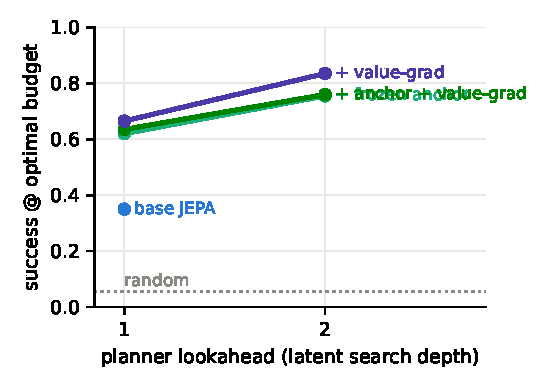
\includegraphics[width=\linewidth]{figs/lookahead.pdf}
\column{0.44\textwidth}\small
Lookahead $d$ = feasible $d$-step sequences (capped), scored at the
imagined end state; no retraining. Depth curves are single-seed; the
depth-1 anchors carry $\pm$0.03--0.05 seed bands (leaderboard slide).\\[4pt]
All recipes converge to $\approx$0.96--0.97 by depth 4 --- the residual
is the deep-chain failure mass (Result on failures), not search.\\[4pt]
Base JEPA: $0.35\to0.87$ (depth 3); \texttt{mono\_hi}
$0.655\to0.97$ (depth 6). The \texttt{rank\_k2} dip at depth 2 is the
calibration anomaly; cost ranking (brown) removes it and dominates at
every depth.
\end{columns}
\end{frame}

\begin{frame}{Result 3 --- encoder--predictor co-adaptation, measured}
\claim{Pure state-prediction JEPA \emph{removes} outcome information that was
linearly present at initialization; a frozen outcome anchor prevents it.}
\begin{columns}
\column{0.52\textwidth}
\centering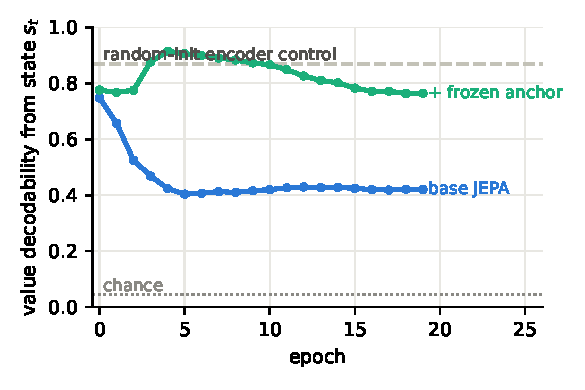
\includegraphics[width=\linewidth]{figs/collusion.pdf}
\column{0.46\textwidth}\small
Probe: linear decodability of the just-computed value (23 classes) from
$s_t$, val split.\\[4pt]
Both loss sides are learned; EMA targets \emph{trail the online encoder}, so
deleting a hard-to-predict feature lowers the loss --- stop-grad does not pin
content.\\[4pt]
Consequence in \texttt{base}: answer decodable from the terminal state
at only 0.26 (random-init control: 0.65).
\end{columns}
\end{frame}

\begin{frame}{Result 4 --- latent arithmetic under a fixed outcome target}
\claim{With $\mathcal L_{\text{chunk}}$, the predictor computes outcomes it
never observes: value decodability from \emph{predicted} latents doubles the
random-encoder control.}
\begin{columns}
\column{0.55\textwidth}
\centering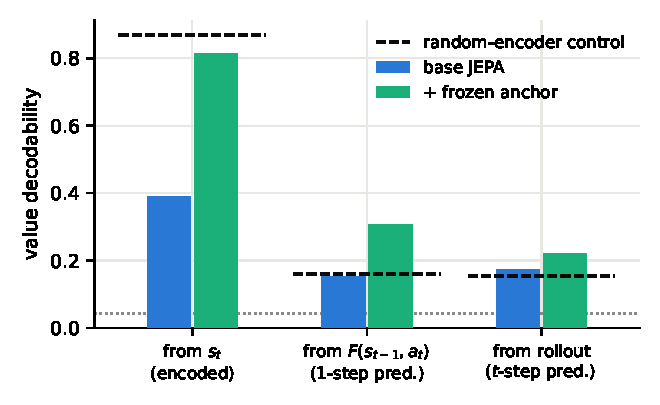
\includegraphics[width=\linewidth]{figs/arithmetic.pdf}
\column{0.43\textwidth}\small
Dashed = random-init encoder control (surface memory, no computation);
dotted = chance $1/23$.\\[4pt]
From $F(s_{t-1},a_t)$: baseline 0.15 ($=$ control) $\to$ fixed outcome target
\textbf{0.31}.\\[2pt]
Answer from terminal state: $0.26 \to \mathbf{0.98}$.\\[2pt]
Full-trace open-loop rollout: 0.22 (error compounds; matches Result 2's
need for re-encoding).
\end{columns}
\end{frame}

\begin{frame}{Result 5 --- the goal energy must be learned (LeWM test)}
\claim{Raw latent distance to the oracle goal state plans barely above
random; the trained value head is the energy that works.}
\begin{columns}
\column{0.5\textwidth}
\centering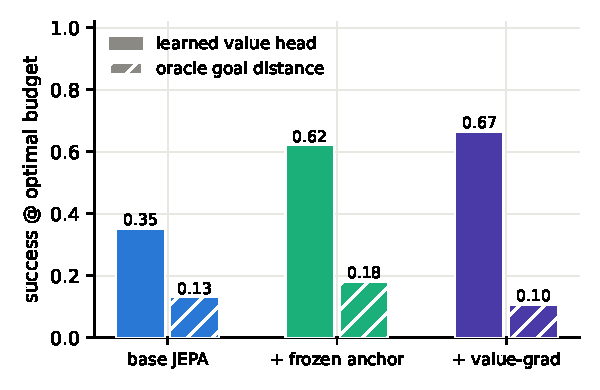
\includegraphics[width=\linewidth]{figs/energy.pdf}
\column{0.48\textwidth}\small
Oracle goal = encoded terminal state of the \emph{true} solution (planner
gets it for free --- upper-bound diagnostic).\\[4pt]
Scoring $\|\mathrm{LN}(\hat s)-\mathrm{LN}(s_{\text{goal}})\|_1$:
latent baseline 0.13, fixed outcome target 0.18, end-to-end value shaping
0.105 (distractor rates $\approx$ random).\\[4pt]
$\Rightarrow$ \emph{unregularized} JEPA geometry is not a distance-to-goal
metric. Result 7 shows temporal straightening fixes exactly this.
\end{columns}
\end{frame}

\begin{frame}{Result 6 --- displacement decoding ablation; stability}
\claim{Our hybrid displacement decoder is useful for planning, but this is
not an exact replication of Delta-JEPA's raw-action reconstruction objective.}
\centering\small
\begin{tabular}{lcccc}
\toprule
 & success@opt & success@slack2 & distractor rate & op from $\Delta s$\\
\midrule
\texttt{base} & \textbf{0.35} & \textbf{0.75} & 0.28 & 1.00\\
\texttt{no\_delta} & 0.15 & 0.51 & 0.40 & 0.98$^*$\\
\bottomrule
\end{tabular}

\smallskip{\scriptsize $^*$Operation type stays decodable (it correlates with surface
features) but transitions lose the \emph{action-discriminative} structure the
planner needs.}
\medskip

\textbf{Stability} (all runs): per-dim state std $\approx 1.03$, RankMe
effective rank 220--243 / 256, no collapse; VICReg + EMA sufficed, discrete
codes (FSQ) not needed. Delta-JEPA decodes the observed continuous action from
$s_{t+1}-s_t$ with MSE and trains end-to-end without EMA or a distribution
regularizer. Here the targets are an operation label and an EMA intent
embedding; operation CE is therefore explicit symbolic action-type supervision.
\end{frame}

\begin{frame}{Result 7 --- temporal straightening makes raw geometry plannable}
\claim{The curvature loss (arXiv:2603.12231) turns latent distance into a
progress metric: goal-distance planning goes $0.15\to0.43$ @optimal
($0.52\to0.85$ @slack 2) --- but it \emph{trades off} against the value head.}
\begin{columns}
\column{0.52\textwidth}
\centering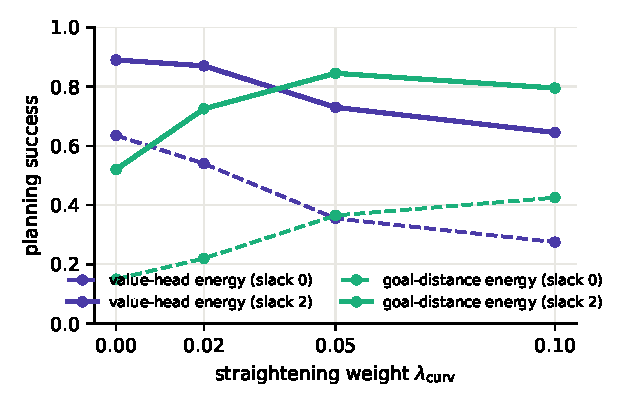
\includegraphics[width=\linewidth]{figs/straighten_tradeoff.pdf}
\column{0.46\textwidth}\small
Dose-response over $\lambda_{\text{curv}}\in\{0,.02,.05,.1\}$ (all on the
fixed-outcome, end-to-end value model):\\[2pt]
\begin{tabular}{lcccc}
\toprule
 & 0 & .02 & .05 & .1\\
\midrule
velocity $\cos$ & $-.25$ & $-.01$ & .42 & .67\\
corr($d^{\text{goal}}$, remaining) & .73 & .75 & .80 & .86\\
value probe from $s_t$ & .89 & .89 & .74 & .43\\
\bottomrule
\end{tabular}\\[4pt]
Geometry improves exactly as content decodability degrades;
$\lambda=.05$ is the raw-geometry sweet spot.
\end{columns}
\end{frame}

\begin{frame}{Result 8 --- two energies, one metric: the content--geometry
trade-off}
\claim{Straightening buys geometry planning, the goal-monotonicity constraint keeps
content and sets the value-planning record; geometry needs JEPA losses, not
value labels.}
\centering\small
\begin{tabular}{lcc|cc}
\toprule
 & \multicolumn{2}{c|}{goal-distance energy} &
   \multicolumn{2}{c}{value-head energy}\\
run & @opt & @slack2 & @opt & @slack2\\
\midrule
\texttt{combo} ($\lambda=0$) & 0.15 & 0.52 & 0.635 & 0.89\\
\texttt{straight\_mid} ($\lambda{=}.05$) & 0.365 & \textbf{0.845} & 0.355 & 0.73\\
\texttt{mono\_hi} (hinge w2 m.05) & 0.255 & 0.68 & \textbf{0.655} & \textbf{0.935}\\
\texttt{mono\_novalue} (\emph{no} $V$) & 0.20 & 0.65 & --- & ---\\
\texttt{value\_only} (\emph{no} JEPA) & 0.06 & --- & 0.075 & 0.43\\
random & 0.06 & 0.095 & 0.06 & 0.095\\
\bottomrule
\end{tabular}

\medskip\small
\textbf{Three readings.} (i) One latent metric cannot currently maximize
both energies --- a learned \emph{projection head} for the geometric energy
is the obvious fix (tested in Result 10: it softens but does not remove the
trade-off). (ii) A model with \textbf{no value head} still plans at
0.65 @slack 2 from pure geometry. (iii) \texttt{value\_only}'s
geometry is \emph{exactly random}: planning-relevant structure comes from
the JEPA objectives, not the value labels.
\end{frame}

\begin{frame}{Result 9 --- the predictor is counterfactually grounded
(direct audit)}
\claim{From each state we enumerate \emph{all} feasible actions, predict
their next-state latents, and check against symbolic execution the model
never saw: $F(s,a)$ is correct per action, and displacement decoding / fixed
outcome targets are what ground it.}
\begin{columns}
\column{0.54\textwidth}
\centering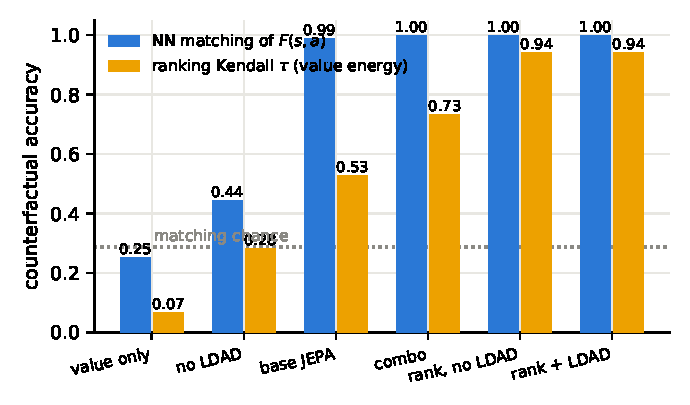
\includegraphics[width=\linewidth]{figs/audit.pdf}
\column{0.44\textwidth}\small
\textbf{Audit metrics} (100 episodes, val):
nearest-neighbor \emph{matching} of $F(s,a_i)$ to the executed-and-encoded
true next states; Kendall $\tau$ of the value energy vs.\ true
post-action remaining steps.\\[3pt]
Training data shows \textbf{one action per state} --- grounding comes from
cross-problem generalization alone.\\[3pt]
Shuffled-action control: matching 0.30 $\approx$ chance. RSA of pairwise
next-state geometry: 0.93 (base+LDAD) vs 0.48 (no LDAD).
\end{columns}
\end{frame}

\begin{frame}{Result 10 --- counterfactual ranking: the strongest lever}
\claim{Hinge-ranking K alternative actions per state by symbolic outcome
nearly closes the gap to the oracle; K=2 suffices; it can replace LDAD but
not data diversity; it trades search-depth calibration for 1-step precision.}
\centering\small
\begin{tabular}{lcccc}
\toprule
 & @opt & @slack2 & @opt look-2 & value $\tau$ \\
\midrule
\texttt{combo} & 0.635 & 0.89 & 0.76 & 0.73\\
\texttt{rank\_k2} & 0.910 & 0.985 & 0.85 $\downarrow$ & 0.94\\
\texttt{rank\_k4} & 0.925 & 0.98 & 0.85 $\downarrow$ & 0.94\\
\texttt{rank\_k4} \emph{no LDAD} & 0.875 & 0.965 & --- & 0.94\\
\texttt{combo} \emph{no LDAD} & 0.48 & 0.805 & --- & 0.69\\
\textbf{preference + goal monotonicity} & \textbf{0.905} & \textbf{0.99}
 & --- & \textbf{0.96}\\
\bottomrule
\end{tabular}

\medskip\small
$\downarrow$ lookahead-2 \emph{hurts} ranking models (0.91$\to$0.85) while
helping regression values (mono\_hi 0.655$\to$0.735): the margin loss
perfects 1-step ordering but distorts $V$'s absolute scale that multi-step
cost sums need. Preference learning + goal monotonicity also has the best raw geometry
($\tau_{\text{goal}}$ 0.82, oracle-goal planning 0.655, no curvature loss).
Seed replicates: rank\_k2 0.885--0.91 @opt, 0.98--0.985 @slack2.
\end{frame}

\begin{frame}{Result 11 --- data-scale trend (coverage and compute confounded)}
\claim{Performance increases with the procedural corpus size, but the original
sweep also changes optimizer updates; it is evidence for a scale trend, not a
clean causal estimate of data diversity.}
\begin{columns}
\column{0.5\textwidth}
\centering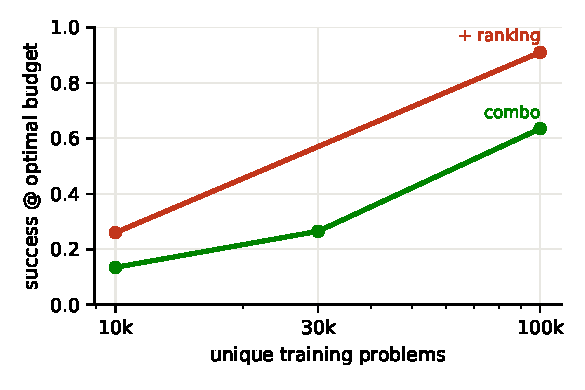
\includegraphics[width=\linewidth]{figs/datascale.pdf}
\column{0.48\textwidth}\small
Fixed 20 epochs: 10k, 30k, and 100k imply approximately 1.6k, 4.7k, and
15.6k optimizer updates, respectively.\\[2pt]
\begin{tabular}{lccc}
\toprule
problems & 10k & 30k & 100k\\
\midrule
combo @opt & 0.135 & 0.265 & 0.635\\
+ ranking & 0.26 & --- & 0.91\\
matching & 0.82 & 1.00 & 1.00\\
value $\tau$ & 0.22 & 0.44 & 0.73\\
\bottomrule
\end{tabular}\\[4pt]
Matching survives small data; \emph{ranking quality} does not --- the
predictor stays roughly right, the energy loses discrimination.
Within-trace variation matters too: no distractors $\Rightarrow$
0.635$\to$0.415. A compute-matched fresh-stream rerun is now required.
\end{columns}
\end{frame}

\begin{frame}{Result 12 --- cross-horizon calibration and macro transitions}
\claim{Plain ranking breaks lookahead (0.91$\to$0.85); two independent
fixes exist, and they don't stack because they repair the same defect.}
\centering\small
\begin{tabular}{lcccc}
\toprule
 & look-1 & look-2 & look-3 flat & look-3 $F_{\mathrm{hi}}$\\
\midrule
\texttt{rank\_k2} & 0.910 & 0.850 $\downarrow$ & 0.915 & \textbf{0.970}\\
\texttt{rank\_cal} (+ cross-horizon calibration) & 0.905 & \textbf{0.945} & --- & 0.915\\
preference + monotonicity + calibration & 0.910 & 0.945 & --- & 0.915\\
\bottomrule
\end{tabular}

\medskip\small
\textbf{Cross-horizon calibration}: rank full MPC costs across depths — executed 2-step
continuation ($2+V(F^2)$) vs 1-step alternatives ($1+V(F(a'))$); zero new
data. \textbf{Macro jumps}: score 3-step sequences with one
$F_{\mathrm{hi}}$ call — worse \emph{fidelity} than $F^3$ (matching
0.62--0.70 vs 0.77--0.91) but stays on $V$'s training distribution.
1000-episode: rank\_cal look-2 = 0.946 vs hier 0.931 — calibration wins
once you have it; macro jumps are the no-retraining workaround.
Train-side hierarchy loss: neutral (\texttt{combo\_nohier} 0.670/0.910).
\end{frame}

\begin{frame}{Result 13 --- the non-symbolic value head (headline)}
\claim{Shape the metric with goal monotonicity, distill it into $V$, add preference learning:
best planner with no numeric value labels anywhere.}
\centering\small
\begin{tabular}{llcc}
\toprule
run & energy supervision & @opt & @slack2\\
\midrule
scalar value + preference + calibration & \emph{numeric} + order & 0.91 $\pm$ .01 & 0.995\\
\textbf{\texttt{mono\_distill\_rank}} & \textbf{binary only (geometric $V$)}
 & \textbf{0.90 $\pm$ .03} & \textbf{0.98 $\pm$ .01}\\
\texttt{mono\_hi} & \emph{numeric} regression & 0.63 $\pm$ .05 & 0.91 $\pm$ .02\\
\texttt{mono\_distill} & binary (no ranking) & 0.57 $\pm$ .05 & 0.89\\
\texttt{mono\_lf\_distill} & \emph{none} (all-steps hinge) & 0.355 & 0.775\\
\texttt{geometric} & \emph{none} (curvature) & 0.300 & 0.715\\
\texttt{distill\_v} & \emph{none, unshaped} (control) & 0.190 & 0.640\\
\bottomrule
\end{tabular}

\medskip\small
Rows 1 vs 2 are the direct \textbf{numeric-vs-geometric} comparison at
matched search settings: the geometric value head ($V$ regressed on the
latent goal distance $d^{\text{goal}}$, ordered by binary-outcome ranking)
matches the scalar-label comparison within seed noise (0.90$\pm$.03 vs
0.91$\pm$.01). Shaping is required: unshaped distillation fails (0.19).
Mean$\pm$std over 3 seeds where shown; single-seed otherwise.
\end{frame}

\begin{frame}{Result 14 --- stability of the hybrid displacement objective}
\claim{Our operation/intent displacement decoder alone does not prevent
collapse; VICReg remains important in the observed-intent architecture. This
does not test Delta-JEPA's exact raw-action objective.}
\centering\small
\begin{tabular}{lcccc}
\toprule
run & EMA & sg & VICReg & result\\
\midrule
\texttt{ldad\_pure} & --- & --- & --- & \textbf{collapse}
 (std .027, rank 80)\\
\texttt{ldad\_pure\_sg} & --- & \checkmark & --- & collapse (0.11 @opt)\\
\texttt{combo\_novic} & \checkmark & \checkmark & --- & 0.27 @opt
 (vs 0.635)\\
\texttt{combo} & \checkmark & \checkmark & \checkmark & 0.635 @opt\\
\bottomrule
\end{tabular}

\medskip\small
This is a negative result for our hybrid decoder, not a negative replication
of arXiv:2606.31232: targets, encoders, and action observability differ.
Also: non-residual predictor $\hat s = \mathrm{MLP}([\mathrm{LN}(s);a])$
performs at least as well as residual (0.710/0.920) — the residual skip is
convenience, not mechanism; LDAD constrains \emph{encoder} displacements,
not predictor outputs, so it is not trivialized by either choice.
\end{frame}

\begin{frame}{Result 15 --- historical outcome-candidate LM diagnostics}
\claim{Outcome-likelihood/reconstruction selectors cluster at 0.47--0.74;
these are strong controls, but their candidate sentences expose computed
consequences and are not information-matched policy baselines.}
\centering\small
\begin{tabular}{llcc}
\toprule
model (selection energy) & params & @opt & @slack2\\
\midrule
sentence-LM (decoder CE) & 7.2M & 0.470 & 0.810\\
sentence-LM+latent tgt (decoder CE) & 7.2M & 0.510 & 0.800\\
sentence-LM+latent tgt (\textbf{latent dist.}) & 7.2M & 0.605 & ---\\
token LM (likelihood, best lr) & 8.2M & 0.670 & 0.910\\
naive JEPA (combo, value head) & 9.1M & 0.635 & 0.890\\
token LM & 25.5M & 0.735 & 0.940\\
\textbf{cross-horizon calibrated JEPA} & 9.1M & \textbf{0.935} & \textbf{0.99--1.00}\\
\bottomrule
\end{tabular}

\medskip\small
All models enumerate the same feasible actions and use the same budget, but
the historical LMs score rendered outcomes whereas JEPA scores outcome-free
intent phrases. Information-matched intent-policy LMs are running. LR was
swept for both families. Note the
within-model dissociation: the sentence-LM's \emph{latent} energy
outranks its own decoder (0.605 vs 0.510) --- selection is a
latent-geometry problem even for reconstruction-trained models.
\end{frame}

\begin{frame}{Result 16 --- objective ablations}
\claim{A constructive sequence identifies anti-collapse and predictive
ingredients; independent removals from the full model localize auxiliary
roles. These are two analyses, not one cumulative ``recipe'' curve.}
\smallskip
\centering\small
\resizebox{\textwidth}{!}{%
\begin{tabular}{lcc|lc}
\toprule
\textbf{constructive sequence} & @opt & eff.\ rank &
 \textbf{removed from full model} & $\Delta$@opt\\
\midrule
ranking only & 0.20 & \textbf{24 (collapse)} & hinge & $-$0.02\\
+ latent prediction & 0.78 & 101 & distilled $V$ & $-$0.04\\
+ VICReg & 0.745 & 234 (healthy) & rollout supervision & $\sim$0\\
+ fixed outcome + displacement decoding & \textbf{0.88$\pm$.004} & 234 &
 hierarchy loss & $\sim$0\\
full geometry-distilled model & 0.90$\pm$.03 & 233 & EMA teacher & $-$0.03\\
 & & & scalar value labels & $\sim$0\\
 & & & residual skip & $+$0.02\\
\bottomrule
\end{tabular}}

\medskip\small
Auxiliary roles remain identifiable: goal monotonicity + geometry-distilled
$V$ defines the non-scalar-value variant (0.36--0.57);
EMA = $+$0.03 over stopgrad+VICReg (which suffice for stability ---
\texttt{noema} 0.605, no collapse); cross-horizon ranking calibrates depth,
but only with the full objective set (five-objective: 0.885 look-2 $<$ 0.900
look-1; full: 0.945). \textbf{Failures remain chain-depth-limited}: 4.4\%
(3--4 steps) $\to$ 59\% (7--9). The edit track shows the same ablation:
the five-objective model reaches 0.455/0.485, matching the full model without
defect labels.
\end{frame}

\begin{frame}{Probes I --- what the discourse state actually is}
\claim{A recency-weighted working memory over a relational scaffold:
structure is objective-independent, content is objective-dependent.}
\begin{columns}
\column{0.46\textwidth}
\centering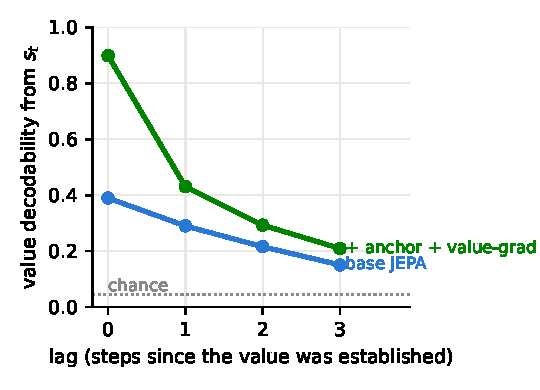
\includegraphics[width=\linewidth]{figs/memory.pdf}
\column{0.52\textwidth}\small
\begin{tabular}{lcc}
\toprule
probe (combo / all recipes) & acc & maj.\\
\midrule
resolved-set member $[s_t;\mathrm{oh}(v)]$ & 0.82 & 0.67\\
ancestor-of-query $[s_0;\mathrm{oh}(v)]$ & 0.76 & 0.56\\
var just resolved (from $\Delta s$) & 0.33 & 0.19\\
query identity (from $s_0$) & 0.19 & 0.16\\
\bottomrule
\end{tabular}\\[4pt]
These rows are \textbf{identical across every training recipe} (base,
no-LDAD, geometry, ranking) while value decodability swings 0.39--0.90:
the encoder learns the scaffold from text alone; the objectives decide
what content survives. Relevance is encoded \emph{relationally} (0.76),
not as a query pointer (0.19).
\end{columns}
\end{frame}

\begin{frame}{Probes II --- emergence, memory, circular code}
\claim{No anticipatory answer computation: the answer appears exactly when
its variable resolves --- and only collusion-free models can hold it.}
\begin{columns}
\column{0.5\textwidth}
\centering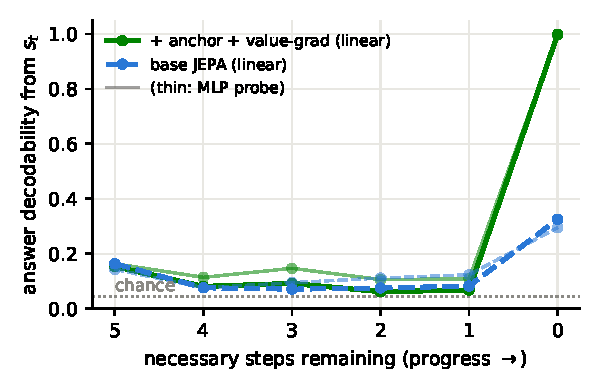
\includegraphics[width=\linewidth]{figs/emergence.pdf}
\column{0.48\textwidth}\small
\textbf{Emergence is a step function}: 0.06--0.18 mid-trace (thin MLP
lines: small nonlinear surplus), 1.00 the moment the query resolves;
\texttt{base} manages only 0.33 even then (collusion).\\[4pt]
\textbf{Memory decays with lag} (Probes I): 0.90 $\to$ 0.43 $\to$ 0.29
$\to$ 0.21 (chance 0.04) --- a working buffer, not a symbol table.\\[4pt]
\textbf{Circular coding}: ridge $R^2$ for $\cos(2\pi v/23)$ from $s_t$:
0.52 (combo) vs 0.20 (base) --- the mod-$p$ value is partly geometric,
and the circle sharpens under the anchor fix.
\end{columns}
\end{frame}

\begin{frame}{Probe suite (fixed outcome target vs. baseline and random encoder)}
\centering\scriptsize
\begin{tabular}{lccc}
\toprule
probe (linear, val split) & \texttt{base} & \texttt{chunkpred} & random-enc\\
\midrule
value of current step from $s_t$ & 0.39 & \textbf{0.81} & 0.87\\
value from $F(s_{t-1},a_t)$ (latent arithmetic) & 0.15 & \textbf{0.31} & 0.15\\
value from open-loop rollout & 0.17 & \textbf{0.22} & 0.15\\
op type from $\Delta s$ & 1.00 & 1.00 & 0.97\\
step goal-relevance from $\Delta s$ & 0.89 & \textbf{0.93} & 0.89\\
remaining steps from $s_t$ & 0.44 & \textbf{0.61} & 0.41\\
resolved count from $s_t$ & 0.97 & 0.92 & 0.95\\
final answer from terminal state & 0.26 & \textbf{0.98} & 0.62\\
answer from prompt alone $s_0$ (should be hard) & 0.035 & 0.05 & 0.04\\
\midrule
value-head MAE (remaining steps) & 0.76 & 0.57 & ---\\
\bottomrule
\end{tabular}

\medskip\small
End-to-end value shaping gives MAE \textbf{0.38} with the same
co-adaptation-resistant probes (state value 0.89).
\end{frame}

\begin{frame}{Scale-up preview --- the hard domain and official iGSM}
\claim{Accuracy degrades sharply on 10--18-step problems; counterfactual
preference learning, capacity, and search depth provide complementary gains.}
\centering\small
\begin{tabular}{lcccc}
\toprule
hard domain (14--24 vars, 10--18 steps) & @opt & @slack2 & look-2 & look-4\\
\midrule
reference recipe (\texttt{combo}, 9M) & 0.000 & 0.070 & 0.035 & 0.175\\
geometry-distilled + cross-horizon calibration (9M) & \textbf{0.120} &
 \textbf{0.445} & 0.105 & 0.150\\
same recipe, 35M & 0.090 & 0.410 & 0.195 & \textbf{0.315}\\
token LM (8M, outcome-candidate score) & 0.010 & --- & --- & ---\\
\bottomrule
\end{tabular}

\medskip\small
Capacity only pays \emph{through search} (35M: 0.09 greedy $\to$ 0.32 at
look-4). And on \textbf{100\%-faithful iGSM} (official facebookresearch
generator vendored; our env drives the reference renderer; solutions pass
the official checker 60/60 med, 99/100 hard): the reference recipe is
near-random (0.245 vs 0.20; probes healthy --- the energy fails, the
pre-ranking signature), 60 epochs don't help (0.235), and
\textbf{counterfactual ranking is again the fix: 0.410 @optimal / 0.735
@slack-2}, and capacity stacks on it (35M: 0.460/0.765, value probe
0.53$\to$0.93) --- the recipe's central mechanism transfers to the
official domain, with the remaining gap to oracle as the next phase's
frontier.
\end{frame}

\begin{frame}{Removing symbolic preference labels: geometric ranking}
\claim{Geometric-advantage ranking (GAR) replaces remaining-step and binary
preference targets with an ordering induced entirely by encoded outcomes.}
\small
At one visited state, execute the trace action and $K$ alternative feasible
actions in cloned environments. Encode each true next sentence with the EMA
encoder and measure its distance to the encoded terminal trace state:
\[
g_i=\|\mathrm{LN}(\bar s^{\mathrm{true}}_{t+1,i})-
        \mathrm{LN}(\bar s_T)\|_1,
\qquad E_i=V(F(s_t,a_i),s_0).
\]
GAR trains $E_i<E_j$ whenever $g_i<g_j$, using only pairwise margins. It uses
no remaining-step count and no symbolic relevance flag.

\medskip
\textbf{Boundary of the claim.} GAR still enumerates feasible actions, renders
counterfactual next sentences, and uses intent phrases. The current GAR jobs
also retain operation-type displacement decoding. It is therefore
\emph{preference-label-free}, not fully action-annotation-free. Two GAR variants
are running; results are not yet included in the tables.
\end{frame}

\begin{frame}{Full variational JEPA over an undifferentiated sentence stream}
\claim{The new model removes intent phrases entirely and represents uncertainty
in both the unobserved transition and the next latent state.}
\small
Prompt and solution sentences form one causal stream; every adjacent pair is a
training transition. Following VJEPA (arXiv:2601.14354), the EMA target encoder
defines a diagonal-Gaussian inference distribution, a target sample is drawn,
and the predictor assigns it likelihood:
\begin{align*}
q_\phi(z_{t+1}\mid x_{\le t+1})&=\mathcal N(\bar\mu_{t+1},
  \mathrm{diag}\,\sigma^2_{q,t+1}),\\
q_\psi(u_t\mid s_t,z_{t+1})&=\mathcal N(\mu^u_q,
  \mathrm{diag}\,(\sigma^u_q)^2),\quad
p_\omega(u_t\mid s_t)=\mathcal N(\mu^u_p,\mathrm{diag}\,(\sigma^u_p)^2),\\
p_\theta(z_{t+1}\mid s_t,u_t)&=\mathcal N(\mu^z_\theta,
  \mathrm{diag}\,(\sigma^z_\theta)^2),\\
\mathcal L&=-\log p_\theta(z_{t+1}^{(q)}\mid s_t,u_t^{(q)})
 +\beta_z\,D_{\mathrm{KL}}(q_\phi\|\mathcal N(0,I))
 +\beta_u\,D_{\mathrm{KL}}(q_\psi\|p_\omega).
\end{align*}
Both predictor and target variances are learned. There is no token decoder,
intent/outcome split, symbolic action target, or feasible-action interface.
This first experiment evaluates representation dynamics and calibration, not
task planning. Stylized and official-iGSM runs are active.
\end{frame}

\begin{frame}{Latent displacement decoding with unobserved actions: factorial test}
\claim{EMA targets require an explicit distribution regularizer here: VICReg
or SIGReg preserves high-rank states, whereas removing EMA produces collapsed
or strongly low-rank states in every cell.}
\small
Delta-JEPA observes $a_t$ and minimizes
$\|D(s_{t+1}-s_t)-a_t\|_2^2$. Our action-free extension instead uses
$\|D(s_{t+1}-s_t)-\sg\,\mu_q^u\|_2^2$. The latter is a consistency constraint:
$q_\psi$ and $D$ can agree on an uninformative code, so we report posterior-mean
standard deviation and effective rank rather than transferring Delta-JEPA's
anti-collapse claim.

\medskip
\centering
\begin{tabular}{lccc}
\toprule
target encoder & no state regularizer & VICReg & SIGReg (LeJEPA)\\
\midrule
EMA target & 2.9 / 1.9 & \textbf{125.1 / 9.2} & \textbf{128.8 / 12.8}\\
shared online target (no EMA/stop-grad) & collapse$^\dagger$ & 2.4 / 2.2 & 16.8 / 7.7\\
\bottomrule
\end{tabular}

\medskip
Each entry is state effective rank / posterior-action-mean effective rank
(maxima 256 / 16) after the same 30k-problem, 10-epoch pilot. $^\dagger$State
std. $=9\!\times\!10^{-4}$ and action-mean std. $=2.5\!\times\!10^{-3}$;
effective rank is misleading at this scale. SIGReg follows LeJEPA's
random-projection normality test. These are collapse diagnostics, not evidence
that the inferred action code is semantically grounded.
\end{frame}

\begin{frame}{Experiments active on July 13, 2026}
\small
\begin{tabular}{p{0.40\textwidth}p{0.27\textwidth}p{0.25\textwidth}}
\toprule
question & runs & status\\
\midrule
Can geometric outcomes replace symbolic preference labels? & GAR + GAR-pure & training\\
How many official-iGSM counterfactuals are needed? & $K=1$ and $K=4$ (with $K=2$ reference) & training\\
Does counterfactual transition data help without ranking? & outcome prediction, $K=1,2,4$ & training\\
Can fully latent actions model a sentence stream probabilistically? & stylized + official iGSM & training\\
How do EMA, VICReg, and SIGReg interact with latent LDAD? & $2\times3$ factorial & completed; diagnostics above\\
\bottomrule
\end{tabular}

\medskip
Only the completed LDAD pilot diagnostics are reported above. The other rows
remain active and should enter result tables only after checkpoint, validation,
and the relevant planning or counterfactual-audit artifact exist.
\end{frame}

\begin{frame}{Honest limitations \& what this is not}
\begin{itemize}\itemsep2pt
  \item Most ablations use the stylized flat-DAG generator. Transfer is tested
        on the vendored official iGSM generator, but not yet at broad language
        variation or natural-text scale.
  \item The reported planning records use observed intent phrases and an
        oracle feasible-action enumerator. The new sentence-stream VJEPA removes
        both interfaces, but does not yet support task planning.
  \item Geometry-distilled values remove scalar remaining-step labels but the
        best completed variant still uses binary relevance and symbolic
        counterfactual ordering. GAR removes those preference labels but still
        uses environment-generated counterfactual outcomes.
  \item Value labels shape only the value head unless \texttt{valgrad};
        operation CE in the hybrid displacement loss is explicit symbolic
        action-type supervision.
  \item Historical data-scale artifacts reused fixed per-index corpora and
        changed optimizer steps with corpus size. Fresh-per-epoch generation is
        fixed for new experiments; the old diversity claim needs a matched rerun.
  \item Text ``generation'' is action selection + template rendering; a
        learned renderer is orthogonal to the world model.
\end{itemize}
\end{frame}

\begin{frame}{Next steps after the active runs}
\begin{itemize}\itemsep2pt
  \item \textbf{Resolve the causal question}: compare $K=1,2,4$
        counterfactual outcome prediction against matched preference-learning
        runs, with identical updates and fresh problems.
  \item \textbf{Audit latent actions}: posterior-mean variance/effective rank,
        transition clustering, uncertainty calibration, and held-out
        next-sentence likelihood for every EMA/regularizer cell.
  \item \textbf{Recover planning without action names}: learn a proposal over
        latent $u_t$ and a separate observation-to-action execution mechanism;
        do not nearest-match against an oracle intent list in the final system.
  \item \textbf{Scale only after the faithful verdict}: use the official iGSM
        $K$ sweep to select counterfactual density, then increase capacity and
        search horizon with a compute-matched protocol.
  \item \textbf{Broaden text}: paraphrases, larger moduli, noisy statements,
        and ultimately non-templated corpora; retain counterfactual audits.
\end{itemize}
\end{frame}

\end{document}
